\documentclass{article}

\usepackage[czech]{babel}
\usepackage{amsmath}
\usepackage[a4paper,top=2cm,bottom=2cm,left=3cm,right=3cm,marginparwidth=1.75cm]{geometry}
\usepackage[nottoc,numbib]{tocbibind}
\usepackage{graphicx}
\usepackage[justification=centering,margin=2cm]{caption}
\usepackage{subfig}
\usepackage{hyperref}

\captionsetup[subfigure]{labelformat=empty}

\title{%
  Simulační studie pro SIS model šíření kapavky\\
  \large T9: Spojitý model v oblasti fyziky a biologie}
\author{Jindřich Vodák, Jakub Vlk}
\date{}

\begin{document}
\maketitle

\newpage
\tableofcontents
\newpage

\section{Úvod}
Jednou z nejsilnějších zbraní lidstva proti šíření nebezpečných nakažlivých chorob není jen vyspělá moderní medicína, ale také schopnost předvídat chování těchto chorob. I lidský mozek však samozřejmě má své limity, a proto jsou v dnešní době velmi důležité spojité matematické modely, které nám pomáhají simulovat šíření různých nemocí v různých podmínkách. Konkrétně v epidemiologii se hojně používají různé variace kompartmentového modelu známého jako SIR (\emph{susceptible -- infectious -- removed/recovered}). Tento model dělí populaci do tří kompartmentů, a sice náchylné k nemoci (susceptible), nakažené (infectious) a vyřazené z modelu (removed/recovered -- tedy buď uzdravené a mimo riziko další nákazy, nebo zemřelé). Z tohoto modelu vychází mnoho dalších, pokročilejších modelů, jako například SIRD, SIS, SIRV, MSIR, SEIR a dále.

Tato studie se zabývá šířením kapavky v populaci. Vzhledem k tomu, že jde o pohlavní chorobu, budeme rozlišovat populaci dle pohlaví na skupinu mužů a skupinu žen a budeme zkoumat šíření choroby napříč těmito skupinami. K tomu je vhodné využít model SIS, který nám zajistí, že každý vyléčený pacient je přesunut opět to kategorie \emph{susceptible}, neboť vyléčená kapavka nezaručuje žádnou imunitu. Cílem této studie je zjistit, jakým způsobem se choroba šíří v populaci mužů a žen při různé velikosti populace a při různých měrách šíření nákazy a rychlosti léčení.
\newpage

\section{Fakta}
Kapavka (\emph{gonorrhoea}) patří mezi nejrozšířenější pohlavní choroby na světě. Přenáší se prakticky pouze pohlavním stykem, což je jedním z důvodů, proč se její šíření dá oproti jiným chorobám relativně dobře modelovat. Kapavka postihuje především sliznice močové trubice a rozmnožovací soustavy, v některých případech však také oči či sliznice v hrdle. Nemoc může (především u žen) probíhat bez příznaků (asymptomaticky), v opačném případě patří mezi časté příznaky obtíže při močení spojené s řezavou či pálivou bolestí, hnisavý výtok z močové trubice a u žen také například zánět děložního hrdla.

Příznaky a průběh nemoci nejsou pro tuto studii příliš podstatné, proto se jim dále nebudeme věnovat. Důležité ovšem je, že inkubační doba nemoci je poměrně krátká, a to 2-14 dní (resp. u 90\% mužů se nemoc projeví během 5 dní, zatímco u žen inkubační doba často trvá i déle než 2 týdny)\cite{MEFANET}. Další důležitou skutečností je, že u žen je nemoc až v 75\% případů asymptomatická. Tyto skutečnosti budou hrát roli při tvorbě simulačního modelu.

Jak již bylo řečeno, kapavka je jednou z nejrozšířenějších pohlavních chorob na světě. Tento fakt dokládají i čísla -- Světová zdravotnická organizace (WHO) odhaduje, že v roce 2020 přibylo 82 milionů nově nakažených kapavkou mezi 15. a 49. rokem života\cite{World_Health_Organization}. Oproti jiným pohlavním nemocem, jako je například syfilis, nepochází tak velké množství případů kapavky z jiných než heterosexuálních styků. Tohoto faktu využívá i tento model, který proto jiné než heterosexuální styky zanedbává\cite{Wikipedia_2023}.

\begin{figure}[h]
    \centering
    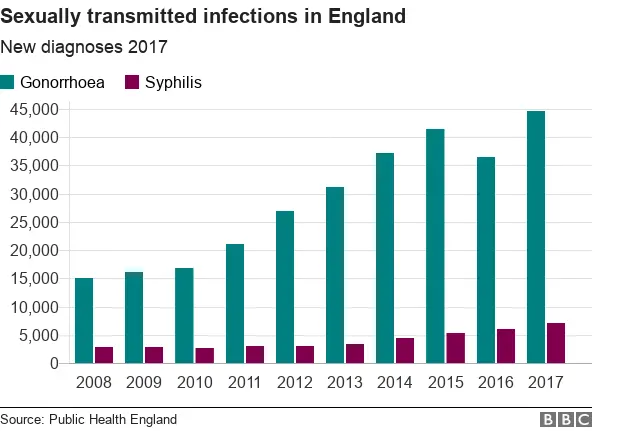
\includegraphics{images/gonorrhoea.png}
    \caption{Nové případy kapavky v Anglii ve srovnání s novými případy nemoci syfilis (Public Health England)}
    \label{fig:enter-label}
\end{figure}

Pro účely modelování šíření této choroby se používá tzv. \emph{maximální ženský/mužský kontaktní koeficient}. Tento koeficient přibližně udává průměrný počet mužů, se kterými má jedna infikovaná žena pohlavní styk, respektive naopak\cite{Kalas_Pospíšil_2001}. Maximální kontaktní koeficient se používá především z důvodu, že je jednodušší jej určit než se zabývat jeho jednotlivými součástmi. Tento koeficient bude použit i v tomto modelu.

V roce 1973 proběhl v USA průzkum, který určil hodnotu maximálního ženského kontaktního koeficientu 1,15 a hodnotu maximálního mužského kontaktního koeficientu 0,98\cite{Kalas_Pospíšil_2001}. Tyto hodnoty budeme používat v tomto modelu.
\newpage

\section{Koncepce modelu}
Jak již bylo řečeno, tento model šíření kapavky bude uvažovat dělení populace dle pohlaví na muže a ženy. Vzhledem ke skutečnosti, že inkubační doba je velmi krátká ve srovnání s dobou aktivní infekčnosti, a rovněž není po vyléčení zaručena žádná imunita vůči nemoci, je SIS model pro tento případ vhodný. Tento model bude uvažovat celkem 4 diferenciální rovnice:
{\large
\begin{align}
\begin{split}
    S'_1&=-\beta_1S_1I_2+\gamma_1I_1\\
    I'_1&=\beta_1S_1I_2-\gamma_1I_1\\
    S'_2&=-\beta_2S_2I_1+\gamma_2I_2\\
    I'_2&=\beta_2S_2I_1-\gamma_2I_2\nonumber
\end{split}
\end{align}
}%

Označme si nyní jednotlivé členy soustavy rovnic:
\begin{align}
\begin{split}
    S_1 &\dots \text{počet mužů náchylných k infekci}\\
    S_2 &\dots \text{počet žen náchylných k infekci}\\
    I_1 &\dots \text{počet infikovaných mužů}\\
    I_2 &\dots \text{počet infikovaných žen}\\
    \beta_1 &\dots \text{koeficient šíření nákazy ve skupině mužů}\\
    \beta_2 &\dots \text{koeficient šíření nákazy ve skupině žen}\\
    \gamma_1 &\dots \text{rychlost léčení infikovaných mužů vztažená na jednotku velikosti populace}\\
    \gamma_2 &\dots \text{rychlost léčení infikovaných žen vztažená na jednotku velikosti populace}\nonumber
\end{split}
\end{align}

Předpokládáme, že $S_1+I_1=N_1$, $S_2+I_2=N_2$, kde $N_1$ je celková populace mužů uvažovaná v modelu a $N_2$ celková populace žen. Dále uvažujeme, že koeficienty $\beta_1, \beta_2, \gamma_1, \gamma_2$ jsou kladné. Z důvodu, že příznaky onemocnění se mnohem výrazněji projevují u mužů než u žen, platí $\gamma_1>\gamma_2$ (výraznější příznaky znamenají, že se muži začínají léčit dříve než ženy).

Určování koeficientů $N_1, N_2, \beta_1, \beta_2, \gamma_1, \gamma_2$ je v praxi velmi obtížné. Obzvlášť koeficient $\gamma_2$ se špatně odhaduje, neboť je u žen častý asymptomatický průběh choroby, díky čemuž je období infekčnosti u žen velmi variabilní. Proto se využívá výše zmíněný mužský a ženský kontaktní koeficient. V tomto modelu mohou nastat dva případy:
{\large
\begin{align}
    \label{eq:1}
    \frac{\beta_1N_1}{\gamma_2}\cdot\frac{\beta_2N_2}{\gamma_1}>1\\
    \frac{\beta_1N_1}{\gamma_2}\cdot\frac{\beta_2N_2}{\gamma_1}<1
\end{align}
}%
kde:
\begin{align}
\begin{split}
    \frac{\beta_1N_1}{\gamma_2} &\dots \text{maximální ženský kontaktní koeficient}\\
    \frac{\beta_2N_2}{\gamma_1} &\dots \text{maximální mužský kontaktní koeficient}\nonumber
\end{split}
\end{align}
Tento model se bude zabývat případem \ref{eq:1}, jelikož využívá údaje z průzkumu uvedeného ve druhé kapitole -- tedy $\frac{\beta_1N_1}{\gamma_2}=1,15$ a $\frac{\beta_2N_2}{\gamma_1}=0,98$, přičemž součin těchto koeficientů se rovná 1,127. V tomto případě jsou podmínky pro koeficienty stanoveny takto:
{\large
\begin{align}
\begin{split}
    \gamma_1+\gamma_2&>0\\
    \gamma_1\gamma_2-\beta_1\beta_2N_1N_2&<0\nonumber
\end{split}
\end{align}
}%

V experimentech budou použity různé hodnoty těchto koeficientů, ovšem takovým způsobem, aby byly splněny všechny uvedené podmínky. V takovém případě bude zajištěno, že je model stabilní.
\newpage

\section{Experimenty}
V rámci experimentů budeme provádět simulaci s různými počátečními podmínkami a výsledky budeme vzájemně porovnávat. Budeme monitorovat vývoj šíření nákazy během období 60 dní. Experimenty jsou navzájem propojeny, takže každý experiment vyjma prvního nějakým způsobem vychází z experimentu přímo předchozího.

\subsection{Experiment 1 -- Prvotní stav}
První experiment provedeme s následujícími počátečními podmínkami:
\begin{align}
\begin{split}
    S_1&=14500\\
    I_1&=500\\
    S_2&=14200\\
    I_2&=100\\
\end{split}
\begin{split}
    \beta_1&=0,00002683333\\
    \gamma_1&=0,7\\
    \beta_2&=0,00005716666\\
    \gamma_2&=0,35\nonumber
\end{split}
\end{align}
Snadno ověříme, že:
\begin{align}
\begin{split}
    0,7&>0,35,\\
    0&<0,7+0,35,\\
    0&>0,7*0,35-0,00002683333*0,00005716666*15000*14300\nonumber
\end{split}
\end{align}
Pro zjednodušení budeme ověřování podmínek v následujících experimentech vynechávat a budeme předpokládat, že jsou splněny.

Po dokončení simulace získáváme tyto hodnoty:
\begin{figure}[h]
    \centering
    \subfloat[\centering]{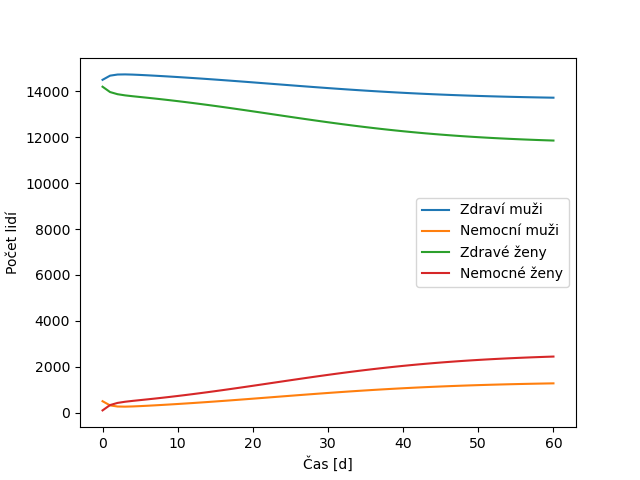
\includegraphics[width=7.0cm]{images/e1/all_vals.png}}
    \qquad
    \subfloat[\centering]{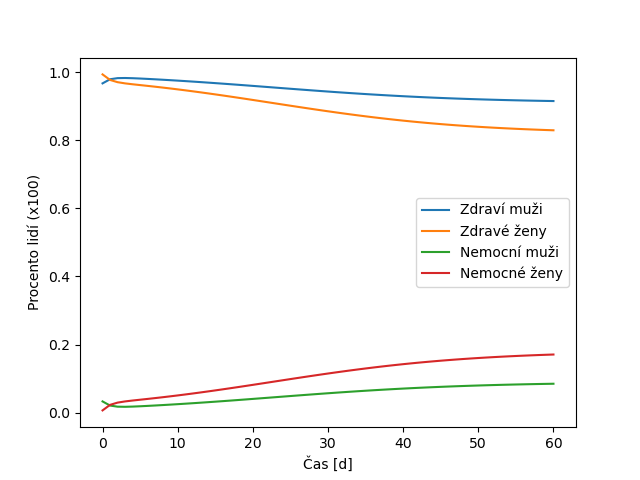
\includegraphics[width=7.0cm]{images/e1/procents.png}}
\end{figure}
\begin{figure}[h]
    \centering
    \subfloat[\centering]{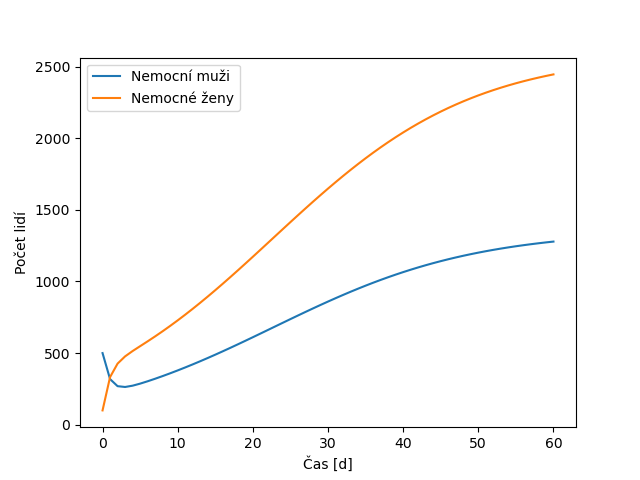
\includegraphics[width=7.0cm]{images/e1/ill.png}}
    \qquad
    \subfloat[\centering]{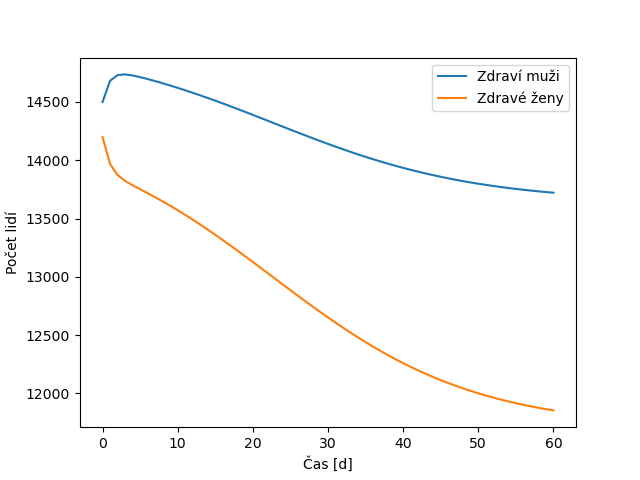
\includegraphics[width=7.0cm]{images/e1/not_ill.png}}
\end{figure}

Vidíme, že při těchto podmínkách počet nemocných žen při těchto podmínkách narůstá výrazně rychleji než počet nemocných mužů.
\newpage

\subsection{Experiment 2 -- Snížení hodnot koeficientů}
Ve druhém experimentu nebudeme nijak měnit stav populace, pouze upravíme (snížíme) oba $\gamma$ i $\beta$ koeficienty. Tím simulujeme stav nižší nakažlivosti a zároveň nižší rychlosti léčení:
\begin{align}
\begin{split}
    S_1&=14500\\
    I_1&=500\\
    S_2&=14200\\
    I_2&=100\\
\end{split}
\begin{split}
    \beta_1&=0,00000383333\\
    \gamma_1&=0,1\\
    \beta_2&=0,00000685314\\
    \gamma_2&=0,05\nonumber
\end{split}
\end{align}

A získáváme tato data:
\begin{figure}[h]
    \centering
    \subfloat[\centering]{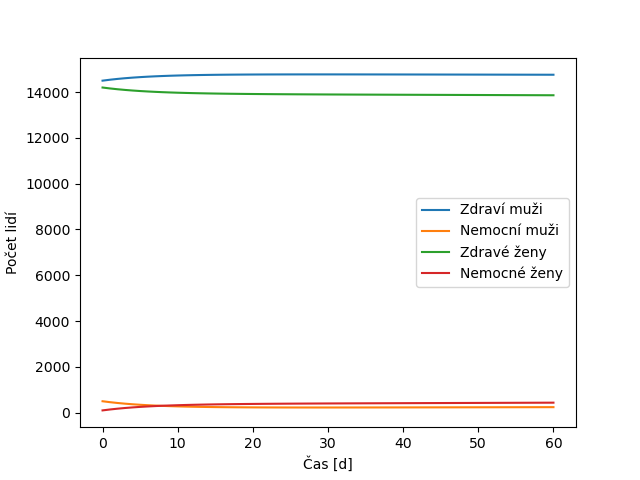
\includegraphics[width=7.0cm]{images/e2/all_vals.png}}
    \qquad
    \subfloat[\centering]{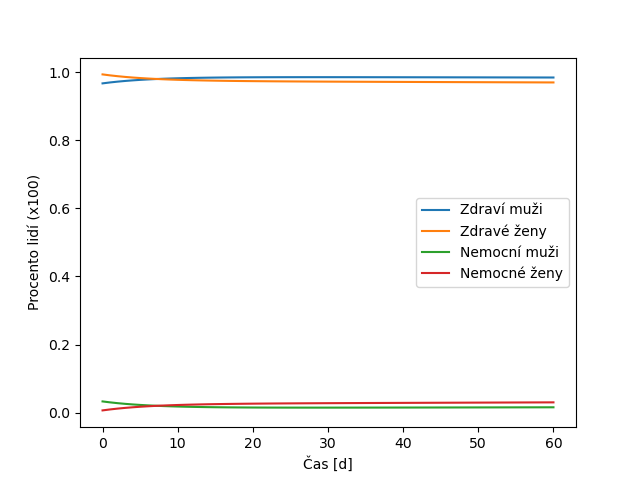
\includegraphics[width=7.0cm]{images/e2/procents.png}}
\end{figure}
\begin{figure}[h]
    \centering
    \subfloat[\centering]{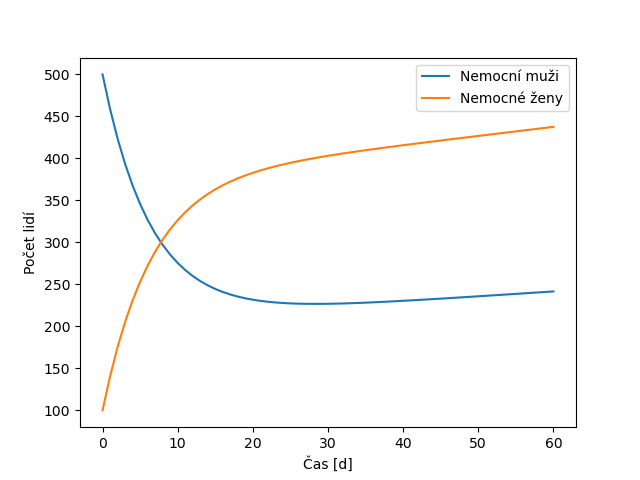
\includegraphics[width=7.0cm]{images/e2/ill.png}}
    \qquad
    \subfloat[\centering]{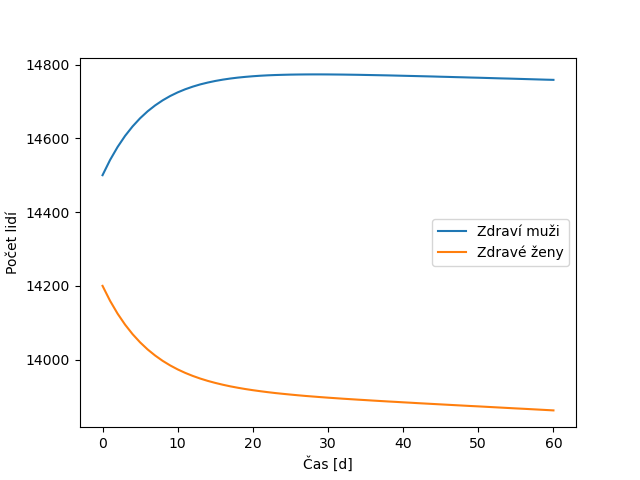
\includegraphics[width=7.0cm]{images/e2/not_ill.png}}
\end{figure}

Vidíme, že změnou obou těchto koeficientů dosáhneme stavu, kdy se systém během 60 dní téměř stabilizuje. Je ovšem také pozoruhodné, že v tomto případě zpočátku velmi prudce narůstá počet nemocných žen, kdežto počet nemocných mužů zpočátku prudce klesá. Je tedy zřejmé, že ačkoliv jsou hodnoty koeficientů značně odlišné než v prvním experimentu, ženy se nakazí rychleji.
\newpage

\subsection{Experiment 3 -- Změna stavu populace}
Ve třetím experimentu nezbývá než změnit stav populace. Ve dvou předešlých experimentech se nákaza šířila výrazně rychleji mezi ženami než mezi muži. Příčinou tohoto může být vyšší počet infikovaných mužů v počátečním stavu. Pojďme proto upravit počáteční podmínky následujícím způsobem:
\begin{align}
\begin{split}
    S_1&=14900\\
    I_1&=100\\
    S_2&=13800\\
    I_2&=500\\
\end{split}
\begin{split}
    \beta_1&=0,00000383333\\
    \gamma_1&=0,1\\
    \beta_2&=0,00000685314\\
    \gamma_2&=0,05\nonumber
\end{split}
\end{align}

Výsledky jsou zajímavé:
\begin{figure}[h]
    \centering
    \subfloat[\centering]{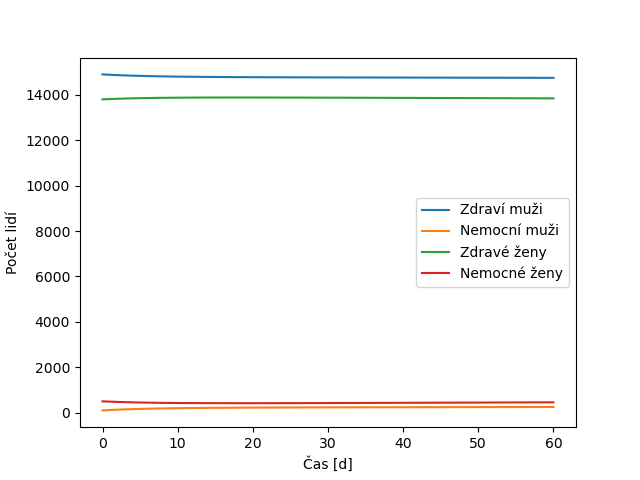
\includegraphics[width=7.0cm]{images/e3/all_vals.png}}
    \qquad
    \subfloat[\centering]{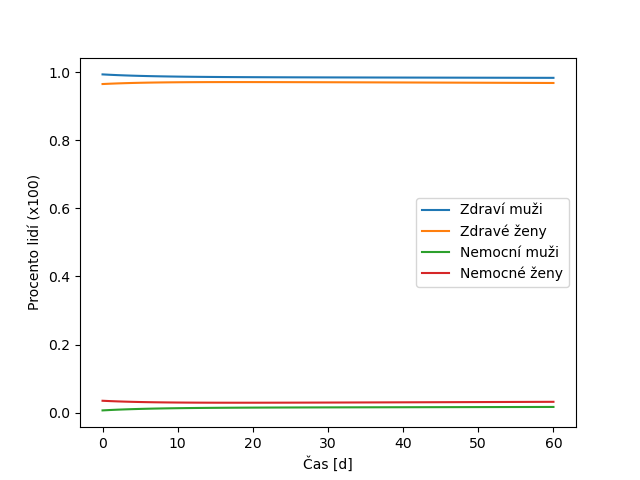
\includegraphics[width=7.0cm]{images/e3/procents.png}}
\end{figure}
\begin{figure}[h]
    \centering
    \subfloat[\centering]{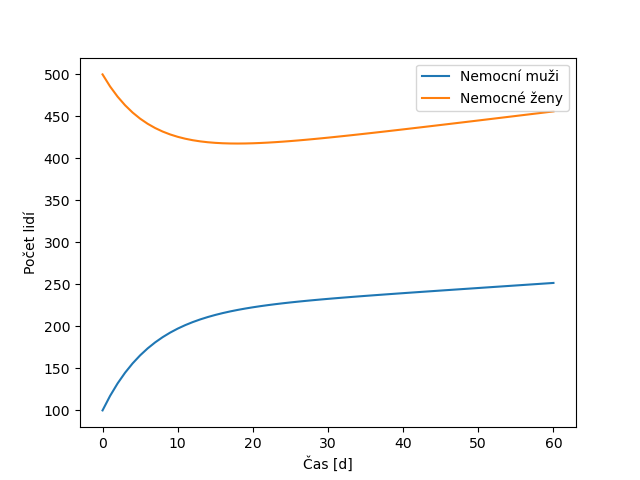
\includegraphics[width=7.0cm]{images/e3/ill.png}}
    \qquad
    \subfloat[\centering]{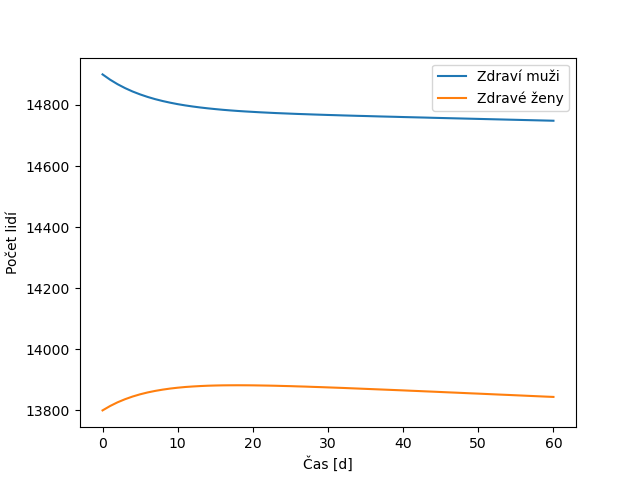
\includegraphics[width=7.0cm]{images/e3/not_ill.png}}
\end{figure}

Je zjevné, že počáteční hypotéza byla správná a změna stavu populace ve prospěch nakažených žen způsobila rychlejší nárůst nakažených mužů. Tento nárůst ovšem není příliš dramatický.
\newpage

\subsection{Experiment 4 -- Zvýšení hodnot koeficientů}
Ve čtvrtém experimentu chceme zjistit, jak bude vypadat vývoj situace s identickými podmínkami populace jako v experimentu 3, ovšem tentokrát se zvýšenými hodnotami koeficientů. Počáteční podmínky stanovíme následovně:
\begin{align}
\begin{split}
    S_1&=14900\\
    I_1&=100\\
    S_2&=13800\\
    I_2&=500\\
\end{split}
\begin{split}
    \beta_1&=0,000069\\
    \gamma_1&=0,95\\
    \beta_2&=0,00006510489\\
    \gamma_2&=0,9\nonumber
\end{split}
\end{align}

Výsledky jsou poměrně překvapivé:
\begin{figure}[h]
    \centering
    \subfloat[\centering]{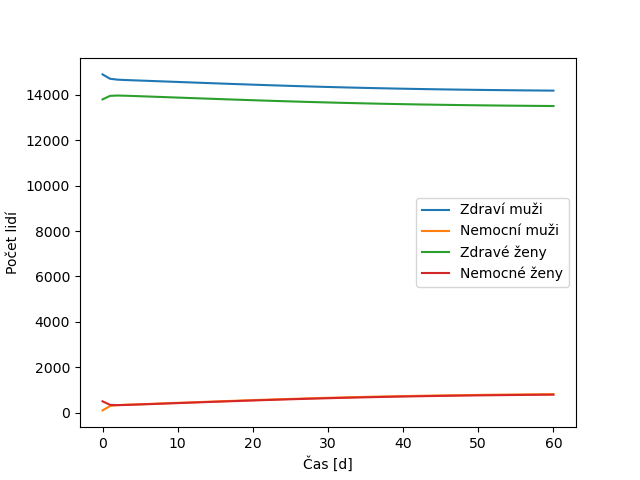
\includegraphics[width=7.0cm]{images/e4/all_vals.png}}
    \qquad
    \subfloat[\centering]{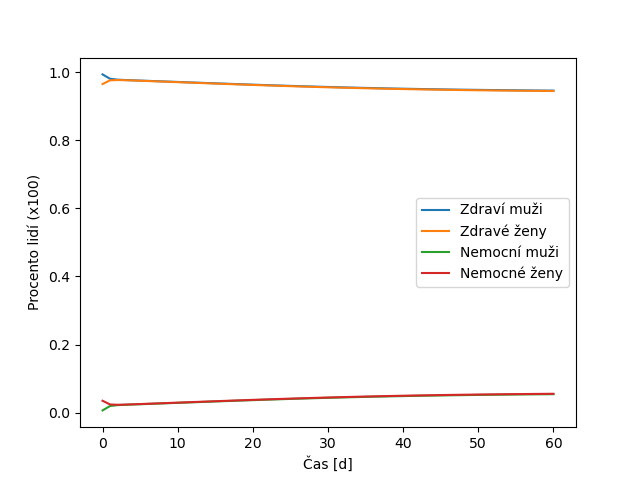
\includegraphics[width=7.0cm]{images/e4/procents.png}}
\end{figure}
\begin{figure}[h]
    \centering
    \subfloat[\centering]{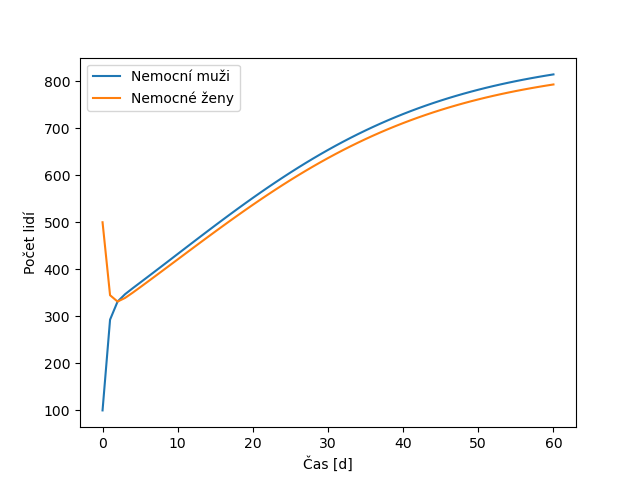
\includegraphics[width=7.0cm]{images/e4/ill.png}}
    \qquad
    \subfloat[\centering]{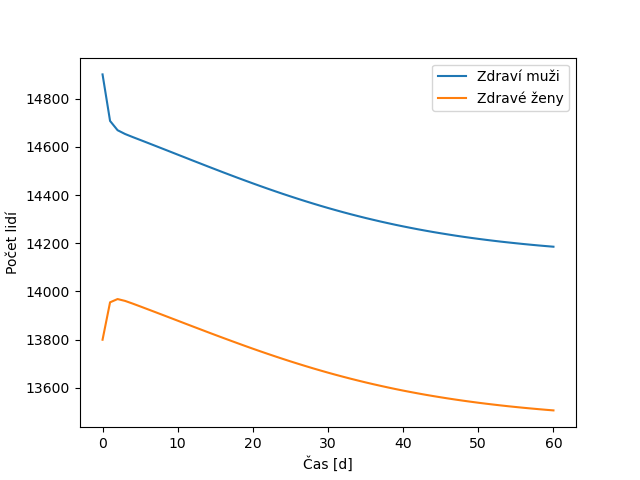
\includegraphics[width=7.0cm]{images/e4/not_ill.png}}
\end{figure}

Pozorujeme drastický nárůst počtu nakažených za den. Toto bylo vzhledem ke zvýšení hodnot koeficientů očekávané. Zajímavé však je, jak rychle počet nakažených žen i mužů zkonvergoval na téměř podobné hodnoty a trend tohoto nárůstu je pro obě pohlaví velmi podobný. Při zvýšení hodnot koeficientů počáteční (relativně) velký rozdíl mezi počtem nakažených mužů a počtem nakažených žen přestává hrát roli.
\newpage

\subsection{Experiment 5 -- Drastická změna populace ve prospěch nakažených žen}
V rámci tohoto experimentu drasticky navýšíme počáteční množství nakažených žen, abychom zjistili, zda se bude výsledný stav dramaticky odlišovat od toho v experimentu 4. Nastavíme počáteční podmínky takto:
\begin{align}
\begin{split}
    S_1&=14900\\
    I_1&=100\\
    S_2&=11000\\
    I_2&=3300\\
\end{split}
\begin{split}
    \beta_1&=0,000069\\
    \gamma_1&=0,95\\
    \beta_2&=0,00006510489\\
    \gamma_2&=0,9\nonumber
\end{split}
\end{align}

Proběhlo tedy navýšení počátečního počtu nakažených žen o 660\%. Získáváme následující data:
\begin{figure}[h]
    \centering
    \subfloat[\centering]{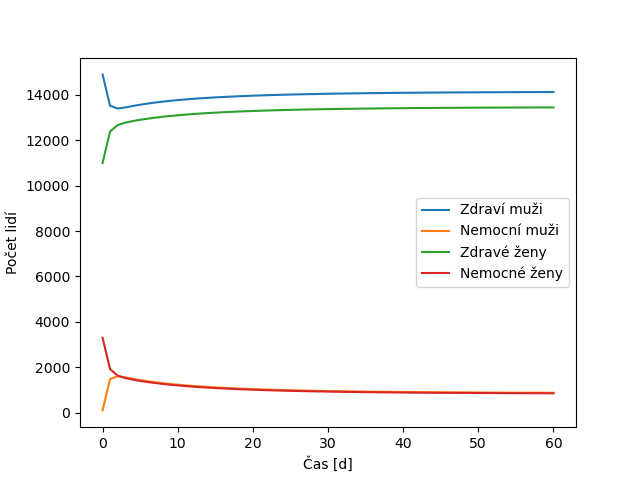
\includegraphics[width=7.0cm]{images/e5/all_vals.png}}
    \qquad
    \subfloat[\centering]{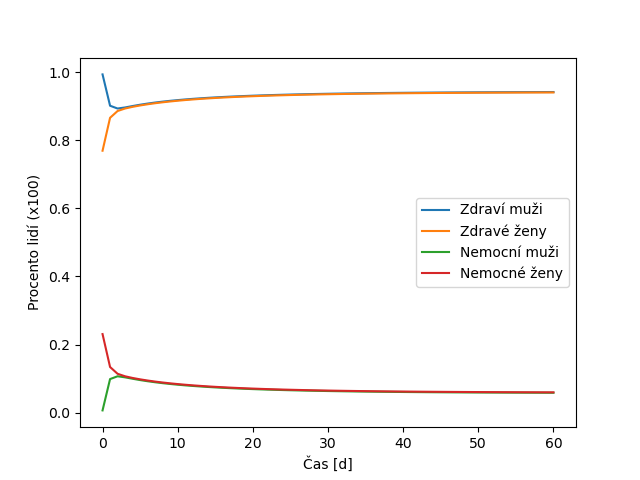
\includegraphics[width=7.0cm]{images/e5/procents.png}}
\end{figure}
\begin{figure}[h]
    \centering
    \subfloat[\centering]{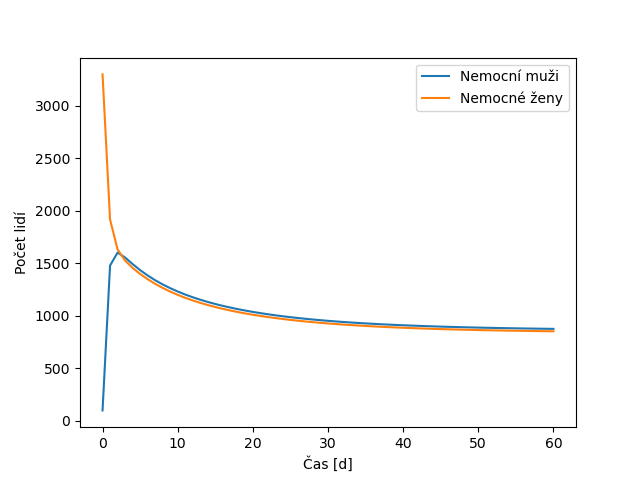
\includegraphics[width=7.0cm]{images/e5/ill.png}}
    \qquad
    \subfloat[\centering]{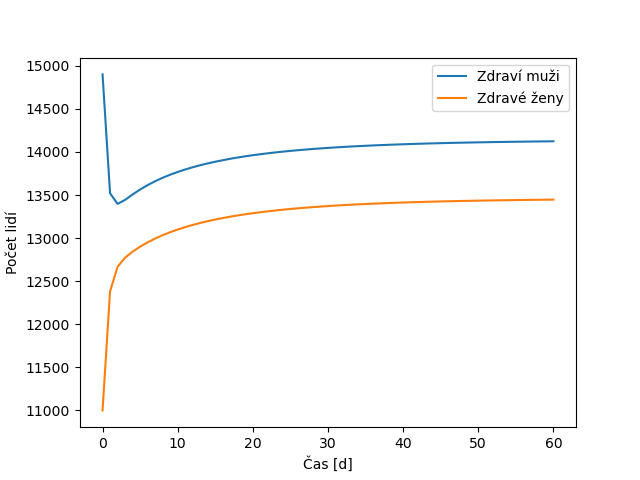
\includegraphics[width=7.0cm]{images/e5/not_ill.png}}
\end{figure}

Jak je vidět, počáteční stav nakažených žen vývoj situace sice výrazně ovlivnil v ohledu celkového stavu šíření/léčení, ale prakticky vůbec neovlivnil podobnost trendů u mužů a u žen. Z toho vyplývá, že na tento trend mají vliv především $\gamma$ a $\beta$ koeficienty, resp. jejich podobnost a výše hodnoty.
\newpage

\subsection{Experiment 6 -- Drastické snížení koeficientu $\gamma_2$}
Cílem posledního experimentu je zjistit, jak se změní trendy přírůstků nakažených žen a mužů při výrazném snížení koeficientu rychlosti léčení infikovaných žen a při zachování populačních podmínek z experimentu 5. Je dobré podotknout, že vzhledem ke vzájemné závislosti koeficientů vycházející z naší definice kontaktních koeficientů tato změna ovlivní i koeficient $\beta_1$. Podmínky změníme následujícím způsobem:
\begin{align}
\begin{split}
    S_1&=14900\\
    I_1&=100\\
    S_2&=11000\\
    I_2&=3300\\
\end{split}
\begin{split}
    \beta_1&=0,0000345\\
    \gamma_1&=0,95\\
    \beta_2&=0,00006510489\\
    \gamma_2&=0,45\nonumber
\end{split}
\end{align}

Výsledky jsou následující:
\begin{figure}[h]
    \centering
    \subfloat[\centering]{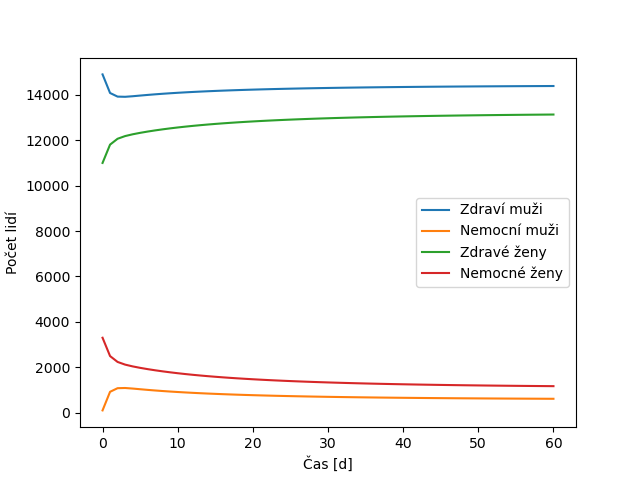
\includegraphics[width=7.0cm]{images/e6/all_vals.png}}
    \qquad
    \subfloat[\centering]{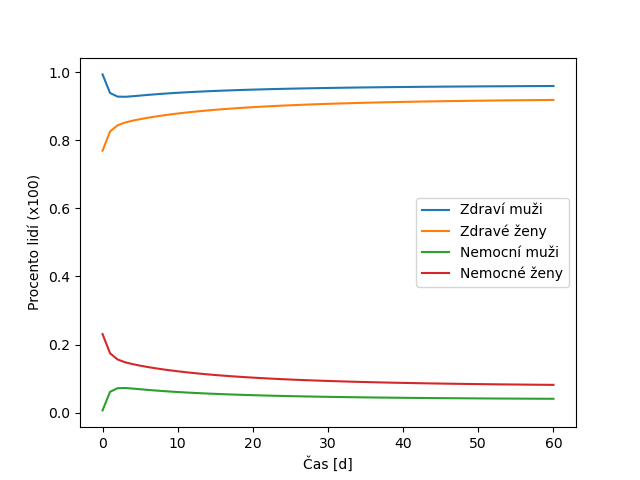
\includegraphics[width=7.0cm]{images/e6/procents.png}}
\end{figure}
\begin{figure}[h]
    \centering
    \subfloat[\centering]{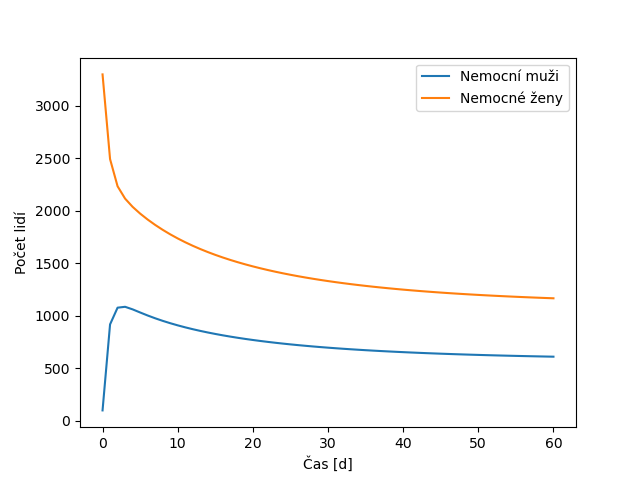
\includegraphics[width=7.0cm]{images/e6/ill.png}}
    \qquad
    \subfloat[\centering]{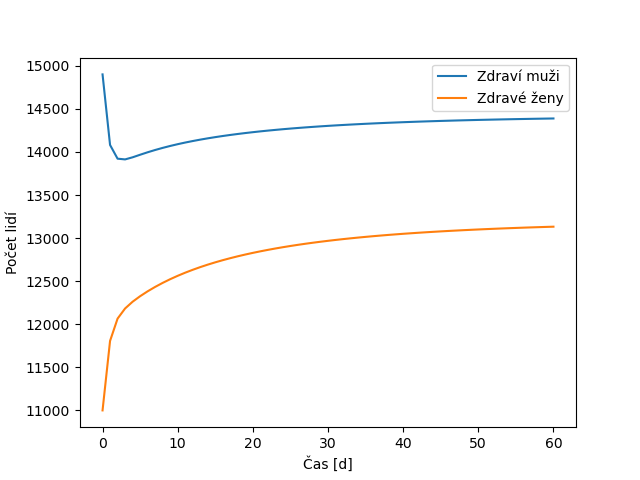
\includegraphics[width=7.0cm]{images/e6/not_ill.png}}
\end{figure}

Tento výsledek je velmi zajímavý, neboť ačkoliv se od sebe křivky nakažených mužů a žen vzdálily, trend vypadá stále velmi podobně jako v minulém případě. Změna koeficientu $\gamma_2$ dle očekávání sníží rychlost léčení u žen, nemá však vliv na samotný trend.
\newpage

\section{Závěr}
Účelem této studie bylo simulovat šíření kapavky v populaci mužů a žen a zjistit, jakým způsobem se tato choroba šíří v různých populačních podmínkách. Bylo zohledněno i různé chování této nemoci s pomocí koeficientů rychlosti šíření a léčení u obou pohlaví. Výsledky ze 6 provedených experimentů nám sdělují tyto poznatky:
\begin{enumerate}
    \item Při podobných mírách nákazy a rychlostech léčení se nákaza šíří rychleji mezi ženami než mezi muži.
    \item Při vysokých mírách nákazy a rovnoměrném rozložení populace dochází k podobným trendům šíření nákazy nehledě na počáteční rozložení nakažených/zdravých jedinců.
    \item Trend šíření choroby v populaci je nejvíce ovlivněn výší nakažlivosti a rychlostí uzdravení u obou pohlaví.
\end{enumerate}
Na závěr je třeba říci, že výsledky této studie vychází z experimentů provedených na konstantní populaci $N_1+N_2=29300$, která tedy nepočítá například s úmrtím pacienta. Vzhledem k tomu, že experimenty modelovaly dobu 60 dní od počátku simulace, dají se případná úmrtí či narození v tomto časovém horizontu zanedbat. Pro přesnější modelování šíření kapavky by však bylo třeba využít složitější a pokročilejší modely.
\newpage

\bibliographystyle{plainurl}
\bibliography{refs.bib}

\end{document}